\documentclass[dvips,letterpaper,12pt]{report}
\usepackage[square,numbers]{natbib}
\usepackage{url}
\usepackage{thesis}
\usepackage{graphicx}
\usepackage{amsmath}
%\numberwithin{equation}{section}
\begin{document}
\chapter{Introduction}

Augmented reality (AR) systems combine standard video inputs with computer-generated objects and
usually provide real-time interaction for the users. 
In general, an augmented reality system can be defined with the following properties \cite{azuma01} :
\begin{itemize}
\item Combination of real and virtual environment
\item Registration (alignment) of real and virtual objects
\item Real-time interaction
\end{itemize}
This concept was pioneered in the 1960s by an American computer scientist named Ivan Sutherland
who created the first head-mounted augmented reality
system with the help of one of his students \cite{azuma01}.

Combining virtual objects and annotations with real
world scenes has proved to be an effective way of conveying information about the surrounding environment to
the user and can be useful in many applications such as gaming, medical surgeries, tourism, and other entertaining, informative or instructional tasks.

Many mobile augmented reality systems have been built over the past decades, from touring machine in 1997 \cite{fei97} 
to google AR glasses which was announced in 2013 \cite{google}; however, most of these prototypes have remained experimental
due to certain difficulties and constraints of using them in practical applications \cite{dras96,liv05}. To name some of the most important constraints
we can refer to:
\begin{enumerate}
\item The requirement of having more advanced hardware and technology
\item Human factors in augmented reality 
\item High demand of computational resources in order to provide a real-time interaction between the user and the system
\end{enumerate}

AR systems overlay 2D or 3D virtual objects on real scenes. Therefore, depending on the application, certain accuracy is required for 
registration of virtual and real objects. There are different approaches to obtain user's location and the position of other objects in the environment.
Tracking sensors such as gyroscope and accelerometer along with video sensors can provide information on the user's position and viewing orientation \cite{azum01}.
In order to find the position of the objects in the scene, a depth map of the surrounding environment at each time would be required. To obtain the depth of the 
objects in the scene several depth sensing technologies can be used such as 3D laser scanner, depth cameras or regular cameras. However, in order to have a mobile AR
system that is easy to carry around, the weight of the whole system will be more of a concern, hence, 3D laser scanners and depth cameras are not good choices for such systems.
Depth cameras, such as Kinect, or DS325 have certain limitation in viewing range (1m-5m) which can worsen in outdoor environments due to various types of noise. 
On the other hand, 3D laser scanners can
generate very accurate depth maps, but they are normally expensive and their price would range from 500\$ to 50,000\$. Therefore, among all these technologies, using several 
cameras to generate a depth map of the surrounding environment seems to be a more efficient approach for outdoor mobile augmented reality systems. {\newline}
However, using several cameras to get the depth map of the scene requires certain conditions to be met, geometrically and computationally. Many researchers have already looked into
this particular problem, i.e, finding the 3D position of the points in the scene from two or multiple views using regular cameras \cite{sze11}. Attempts of these researchers have resulted in
certain techniques in computer vision to find the depth of different points in an environment using one or more stereo pairs taken from slightly different points of view of the same scene.
These techniques are known as {\it Stereo Correspondence} or {\it Stereo Matching} in computer vision \cite{sze11}. Stereo matching has been one of the most studied subjects in computer vision for 
many years now and there are many solutions proposed by researchers to address this problem using different techniques; however, finding the corresponding pixels in stereo pairs with certain level of 
accuracy and in real-time for practical applications still remains a challenging task. {\newline}

% Motivation - Objective - Contributions %
\section {Research Objective}

Our motivation in this research is to study the possibility and usability of combining stereo vision approaches with AR systems considering the most important constraints that AR systems
normally come across. Therefore, we have tried to propose an evaluation scheme that enables us to examine whether using stereo vision
for obtaining 3D position of objects is potentially a practical approach in an augmented reality application. A particular application that we have been considered in
this study, is a 3D mobile augmented reality system in urban settings. 
In fact, our fundamental research question is: \newline

\begin{quote}
\textbf{"Can combination of stereo matching techniques with augmented reality meet the requirements of an AR system?"} \newline
\end{quote}

In order to find the answer to this question, some other questions are raised:
\begin{quote}
\textbf {"How can we evaluate stereo correspondence in an augmented reality framework? What are the important factors we need to consider for this type of evaluation?"} \newline
\textbf {"In a combination of augmented reality with stereo vision, what would be considered as \textbf{\it accurate} depth result?"} \newline
\textbf {"How is the depth perception of surrounding environment in human visual system?"}\newline
\textbf {"What is the standard stereo acuity for human visual system? How would it affect an AR system?"} \newline
\textbf {"What are the requirements to maintain an interactive augmented reality application for the user"} \newline
\end{quote}

In order to pursue our goal in this research, we have designed and implemented a testbed for evaluation of
stereo matching solutions based on specific criteria which will be thoroughly described later in this report.


In the AR system of our interest, the depth map generated from two or multiple camera views will be used as the depth source to determine the position of the objects in the scene when
overlaying virtual objects at different locations and depth levels in the real environment. For our research, we decided to narrow down our study to the effect of using stereo vision
on two of the most important constraints of an AR system mentioned earlier; {\it human factors} and {\it real-time interaction}. {\newline}
Human perception of depth can vary depending on the environment and under different circumstances. Many studies have focused on the evaluation of human perception of depth within different frameworks
and in different applications, such as virtual reality, and augmented reality which have recently attracted more attention \cite{wann95,dras96,liv05,jer05,swa07,kru10}.
These studies show that the viewer perception of depth
is inversely proportional to his/her distance from the object \cite{kru10,swa07,jer05,liv05}. For instance, in \cite{swa07} some experiments are designed to study and evaluate human
perception of distance, which is the absolute depth of the objects from the observer, for an outdoor augmented reality application in urban settings. 
However, what we are more interested in for this research, is the human perception of relative depth in stereo vision, which is the ability to perceive and distinguish 
the depth of different objects relative to each other. This is known as {\it Stereoscopic Acuity} in binocular vision, which is the smallest depth difference between two points 
that can be detected in binocular vision \cite{pfa2000}. More detail about
this metric will be provided in the following chapters.
Therefore, we have investigated standard stereo acuity in human visual system and applied it to our evaluation in order to obtain the smallest detectable depth of 
objects in human binocular vision based on their distance from the observer.

Moreover, providing real-time interaction in an AR system for the user requires the processing time and update rate of the whole system to keep up ideally with the standard video frame rate, 
between 24fps and 
30fps, or higher. 
However, studies show that in practice to build a reasonable interactive augmented world the processing rate should not be less than half of the video frame rate \cite{hertz00}. 
There are different approaches to speed up a system. Acceleration of a system is possible in two ways:
\begin{enumerate}
\item Using more advanced technology and hardware
\item More sophisticated and efficient software design
\end{enumerate}
However, having access to advanced technology and better hardware is not always feasible and even the most advanced technology have some limitation in their memory space and computational capability
which may not meet the requirement for some real-time applications. 
Therefore, we have decided to focus more on the second approach while designing our evaluation system which also looks into the 3rd most important property of
an AR system mentioned earlier, i.e, real-time user interaction. \newline 

One of the most important features that makes our evaluation unique and different from the others is that we have tailored the evaluation process of stereo matching algorithms for an augmented 
reality system. Therefore, we have designed our evaluation testbed within this framework, while keeping in mind the most important properties and constrains of an AR system.
In order to address the speed factor in augmented reality systems we have decided to focus on certain regions of the scene rather than the whole image for generation and evaluation of 
depth values.  
This idea which originates from having a more efficient design for gaining speed up, 
also addresses the computational resources used during the process and may lead to significant system speed up.
It is also known that distinctive features such as {\it edges}, either in RGB or depth images from a scene, play an important role in many computer vision applications, such as object detection and 
tracking, determination of a set of reliable correspondences to build a 3D model that helps with better perception of object locations in 3D space \cite{mart01,sze11}.

Therefore, in an augmented reality application, wrong depth results, especially in those regions, which will lead to erroneous registration of virtual and real objects, 
can be perceived and picked out easier by the human eyes. This may cause poor performance of the system and possibly faulty interaction between 
the user and the augmented world. 
Hence, in this research we have focused more on studying and evaluating the results of stereo correspondence algorithms in particular regions. Since the depth of the objects 
in a scene and their perception by human visual system are more important in the AR application of our interest, we have 
defined these regions to be depth edges and their surrounding region in the scene \cite{liv05,kru10}.
Our hypothesis is that edges, which can also be good indicators of object boundaries and occlusion, are one of the important depth cues for the observer 
to perceive the depth of different objects in the scene \cite{sze11}. 
Moreover, inspection of the regions within a few pixels of the depth edges in the scene would also address the problem of occlusion and depth discontinuity, which are two of
the most challenging regions in stereo matching algorithms \cite{sch02}.
Finding correct depth values in these 
regions can lead to a more accurate combination of virtual and real objects in the scene and therefore a more reasonable augmented world from the user point of view to interact with. \newline
\newline

Since our objective in this research is to study a hybrid system of stereo vision and augmented reality, we have surveyed some of the existing approaches in stereo matching and the
related geometry of 3D reconstruction from stereo pairs. We will go through these concepts and the related works in the field more in the next chapter. 

To evaluate our proposition in this research, we have decided to assess two stereo matching algorithms. These algorithms are:
\begin{enumerate}
\item Semi-global block matching
\item On building an accurate stereo matching system on graphics hardware \cite{mei11}
\end{enumerate}

The first algorithm, also known as SGBM, is a modified version of Semi-global block matching by Hirschmuller \cite{hir08}, 
and has been implemented in Open Source Computer Vision Library (OpenCV) \cite{sgbm}. Therefore, we have used its OpenCV implementation. 
On the other hand, there was no source code available for the second algorithm. For this reason, we have used our own implementation of this solution in the evaluation process, both on CPU and GPU.

The reason we have chosen these two algorithms is that the first method, SGBM, has shown to generate acceptable results within 1-2 seconds on typical test images \cite{hir08} and 
its implementation in OpenCV library has also made its usage more common and easier in applications. The second algorithm, also known as ADCensus \cite{mei11}, was chosen since 
it has been designed in a way that
can be ported to graphics processing unit (GPU) for acceleration and according to the Middlebury evaluation benchmark \cite{mideval}, it is currently ranked as one of the top algorithms for 
stereo matching regardless of the running time.
It should also be noted that this solution uses better and more sophisticated approaches to do stereo matching which makes it superior to many other solutions \cite{mideval}. \newline
For our evaluation, we have used KITTI stereo training dataset as our stereo image data \cite{kitti}. 
Images in this dataset are more realistic since they have been taken from outdoor scenes under different circumstances 
and the ground truth disparity map is also provided for each of them, which is useful in the evaluation process. KITTI Vision project also provides a benchmark and an evaluation table
for different stereo
matching algorithms assessed in real outdoor scenes which makes it more relevant and applicable to an augmented reality application. 
AdCensus does not currently exist in the KITTI evaluation table which is another reason for us to use it in our evaluation.


\chapter{Background and Related Works}
Stereo vision is the concept of viewing a scene (object) in the real world from slightly different
viewpoints at the same time which results in stereo image pairs. Using computer vision techniques, it is possible to extract depth information from stereo
images. This process is called {\it Stereo Matching} or {\it Stereo Correspondence} in computer vision,
which in fact leads to the construction of a
3D model of a scene from two or multiple views by finding corresponding pixels and therefore, their spatial movement within various views of the same scene \cite{sze11}.

Corresponding pixels in stereo images are the ones that represent the same point in the real
world. As it will be seen shortly in more detail, the amount of horizontal motion of such pixels
in stereo pairs, which is referred to as {\it disparity}, is inversely proportional to the
distance from the observer, i.e., depth; however,  estimation of the exact depth of the points requires some
other information as well, such as the position, and the calibration data of the cameras that took the pictures.
While the physical and geometrical approaches to this problem are well understood by researchers in the field, the process of finding the corresponding pixels correctly, yet efficiently
and measuring the disparity to generate a dense depth map still remains a challenging task. \newline

\section{Epipolar Geometry}
Understanding the fundamentals in the underlying geometry of stereo matching helps to better understand the principal idea behind all the methods designed to address this problem, 
thus facilitating the comprehension of 3D model reconstruction from stereo image pairs. Therefore, we will thoroughly describe the basic geometry of stereo matching in this section. \newline
If we consider two cameras that are looking at a particular scene from slightly different view points, a back projection of any point in the 3D space via rays passing through each camera centre
would result in two distinct points on each image plane. For simplicity, we will refer to the point in space as $P$, and its projection on the first (left) and second (right) image planes,
as $P^{'}$ and ${P}^{"}$ respectively. \newline
As a result of $P$'s back projection on the image planes, an important property will emerge between the points and the camera centres, which is coplanarity of all these points. 
This plane, also referred to as {\it epipolar plane}, passes through $P^{'}$, $P^{"}$ and the camera centres, thus intersecting each image plane. 
It should be noted that this property, from which the consequent properties are derived, is the building block of stereo matching methods. 
Let us denote the specified plane by $S$ for further reference. 
Since $S$ passes through the camera centres, it clearly traverses the line 
that connects two camera centres. This line, which is known as the {\it baseline}, intersects each image plane at a point called the {\it epipole}. 
Consequently, the intersection of the plane $S$ and each of the image planes, creates a line called {\it epipolar line} \cite{hart2000}. 
The {\it epipolar line} always passes through the {\it epipole} in the image plane. 
These concepts, illustrated in figure \textbf{FIGURENUM}, constitute the important components of the stereo correspondence geometry. \newline 
(\textbf{FIGURE HERE FOR EPIPOLAR GEOMETRY TERMS}) \newline

Now, we can define the problem of stereo correspondence as a case in which the location of $P^{'}$ in the image plane is known, while the
corresponding point $P^{"}$ is unknown; therefore, the problem can be stated as an attempt to find the correspondence of $P^{'}$ in the second image plane. Based on the aforementioned 
properties, we know that $P^{"}$ is located somewhere on the line, the epipolar line,
created by the intersection of the plane traversing the ray that goes through $P^{'}$ and the first camera centre and the {\it baseline}. This line is in fact, the projection of the ray going
through $P^{'}$ and the first camera centre, on the right image plane. Therefore, the search for the corresponding point, $P^{"}$, will be limited to merely scanning the corresponding 
epipolar line on the second image plane rather than the whole image.

(\textbf {FIGURE  for epipolar planes similar to the figure in multipleview geometry page240}) \newline 
%\begin{figure}{h!}
%\centering
%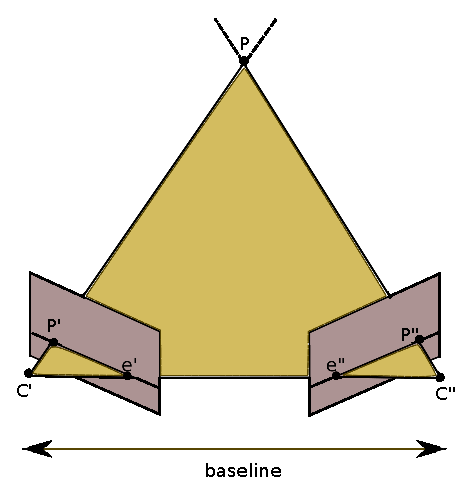
\includegraphics[width=1.5in,height=1.5in]{epipole}
%\end{figure}

It is now apparent that in order to find the correspondence of a particular point $P^{'}$, in the second image plane
the corresponding epipolar line, must first be sought. 
The projection from a point to its corresponding epipolar line can be obtained through certain transformations in space; normally a rotation and translation, \textbf {FIGNUMER}.
For further geometrical calculations, these transformations can be represented
with a matrix that is only dependant on the camera's properties, not the scene \cite{hart2000}.
However, dealing with these transformations while looking for the corresponding points, can increase the complexity of stereo matching algorithms to certain levels \cite{sze11}; therefore, 
in order to avoid this issue, many stereo matching approaches are proposed based on the assumption that image pairs are first warped, i.e. {\it rectified} \cite{sze11}.
This process is known as {\it image rectification} which is basically achieved by first having the cameras rotated in a way that their optical axis, 
the line passing through the camera centre which is perpendicular to the image plane, are parallel to each other; 
i.e. their optical axis is perpendicular to the baseline. Furthermore, it might be necessary to have the cameras tilted so that their {\it y} axis also becomes perpendicular to the optical axis. 
After these two steps, corresponding epipolar lines actually becomes horizontal scanlines \textbf{FIG}. This pre-processing step significantly constrains the process of searching 
for corresponding points and eliminates certain complications in stereo matching algorithms \cite{sze11}. \newline 
Using the rectification model and epipolar geometry described earlier, 
derivation of the geometrical relation through which the depth of a certain point in 3D space 
can be obtained, will be straightforward. This relation is presented as follows \cite{sze11}:
\begin{equation}
d = f\frac{B}{Z}
\end{equation}
where f is the {\it focal length} measured in pixels, B is the {\it baseline}, Z is the {\it 3D depths}, and d is {\it disparity}. The relationship between corresponding pixels in the left
and right images according to disparity {\it d} is also as follows:
\begin{align}
{P}^{"}_{x}={P}^{'}_{x}+d(x,y) \\
{P}^{"}_{y} = {P}^{'}_{y}
\end{align}
Therefore, based on the aforementioned formulas, the depth of points in 3D space can be easily calculated after finding the corresponding pixels in multiple views and consequently their
disparities \cite{bol87,oku93,sch02}.

\section{Stereo Correspondence Algorithms}
A survey of the field shows that the algorithms which address stereo correspondence problem can be roughly divided into two main classes \cite{sch02}. These classifications are commonly known as:
\begin{enumerate}
\item Sparse Correspondence Algorithms
\item Dense Correspondence Algorithms 
\end{enumerate}

In this section, we are going to briefly describe the important specifications of the algorithms belonging to each of these two categories.
\subsection{Sparse Correspondence Algorithms}
Sparse correspondence algorithms, also known as feature-based algorithms, are the early stereo matching methods. In the 1980s, this class of algorithms received considerable attention by
many researchers in computer vision \cite{dhon89}.
In this type of methods, particular features in an image, such as edges, 
points, line segments, or other distinctive features are extracted; therefore, the search for corresponding pixels is only applied to these regions. 
Consequently, algorithms of this
type result in a sparse disparity map \cite{matt89,hsie92, sze11}. The introduction of feature-based algorithms has mainly been motivated by three important factors \cite{bro03,sze11}:
\begin{itemize}
\item Lack of advanced hardware and technology for exhaustive computational tasks 
\item Constraint of the search area in order to find more reliable matches.
\item Image pairs with different illumination, where edges or some other particular features preserve their photometric properties and therefore, are the only regions reliable enough to 
be used for correspondence search.

However, the requirement of having dense depth maps for many applications and also the emergence of efficient {\it dense correspondence algorithms}, have diverted the attention away
from this class of algorithms in the last 20 years.
\end{itemize}

\subsection{Dense Correspondence Algorithms}
Unlike feature-based methods, dense correspondence algorithms try to find the
correspondences for all the pixels in the image, and therefore, result in a dense disparity map. Most recent algorithms and studies have focused on this class of algorithms since many applications 
nowadays, such as graphical rendering, 3D model construction, or augmented reality require a dense depth map of the scene. 
However, this class of algorithms face many challenges that need to be properly
addressed, such as finding the depth values in depth discontinuities, occluded regions and textureless areas \cite{sch02,bro03}.

Dense correspondence algorithms can be classified in two groups based on how they assign
disparities to pixels \cite{sze11}:
\begin{enumerate}
\item Local approaches
\item Global approaches
\end{enumerate}

\subsubsection{Local Approaches} 

Local methods tend to find the disparity of each pixel based on its neighboring pixels. In
other words, the disparity of a pixel is calculated in a finite window containing its neighboring pixels, based on a particular metric, e.g. the intensity values \cite{sch02}.

These methods make an implicit smoothness assumption for the pixels in the search
window, and therefore, assign the same disparity to all the pixels belonging to the same window which could result in incorrect disparity values in slanted surfaces or
depth discontinuities \cite{hirsch02}. This assumption can be considered as one of the major drawbacks of local methods.
Another drawback of local methods is their dependency on the window size \cite{sch02}. A fixed window size can raise certain problems in these algorithms:
\begin{enumerate}
\item If too large of a window size is considered, due to aforementioned smoothness assumption, the algorithm may result in blurry object boundaries and inaccuracy near depth discontinuities.
\item If the window size chosen is too small, the disparity values will be less accurate since little information has been considered for 
finding the correspondences of pixels in the image.
\end{enumerate}

However, a significant advantage of using local approaches is their high speed in finding disparity results.\newline

\subsubsection{Global Approaches}
Unlike local approaches, in global methods the disparity of a pixel depends on the information in
the whole image. Global methods usually include an optimization step of a global energy
function\cite{roy98,bobi99,boyk01,hong10}. In this class of algorithms, an optimal disparity value for each pixel is sought that leads to minimization of a global cost
function that normally combines a data term with an explicit smoothness assumption.

\begin{equation}
E(d)=E_{data}(d)+\lambda E_{smooth}(d)
\end{equation}
The term $E_{data}$ is normally represented as the difference of a common metric, e.g. the photometric property, between the corresponding pixels and is denoted as follows:

\begin{equation}
E_{data}(d) = \sum_{(x,y)}C(x,y,d(x,y))
\end{equation}

where C is a matching cost. The matching cost function can have various definitions depending on the algorithm; however, it is normally defined as sum of absolute difference 
between the intensity of the corresponding pixels in two images \cite{sch02}.

The term, $E_{smooth}$, is the smoothness assumption based on which the disparity values in different regions are refined. The definition of this term can also vary in 
different solutions. $\lambda$ is also a weighting factor, by which the effect of the smoothness assumption in the global function can be controlled in the algorithm \cite{sze11}.
In order to find the minimum of the global function, common approaches in computer science have proved to be particularly useful. 
To name some of these approaches, we can refer to dynamic programming, graph cut, and belief propagation. Many researchers have studied and addressed the problem of stereo matching
by applying one of these approaches \cite{sch02,boy01,boy04,kim05,sun11}.

The major drawback of global approaches is normally their high usage of computational resources and low speed. However, 
they usually result in more accurate disparity values \cite{hirsch02,sze11}. 

It is also worthwhile to mention that in the past 12 years, another group of algorithms have emerged which cannot be explicitly classified in any of the previously mentioned groups.
This group of methods, which are known as {\it Segmentation-based techniques}, first segment the image into regions and then, rather than searching for correspondences per pixel,
they attempt to find the corresponding disparity for each region. A more detailed review of these methods can be found in \cite{sze11}.

\subsection{Edge Detection}

As mentioned earlier in the "Introduction", salient {\it edges} in the scene are one of the important features 
that can be used in many applications, such as object detection, image stitching, or 3D model reconstruction \cite{sze11}.
Due to their importance in defining the boundaries of objects and also their role in occlusion occurrence and depth discontinuities in 3D, we have also focused on employing them in our
evaluation approach; therefore, we have masked our input data based on the detected edges in the scene. 
In order to extract this feature in the images, i.e. edges, we have used 
specific algorithms. Here, we will describe how it is possible to find the most salient edges in the scene using vision techniques and how closely they match the human perception.

When looking at a scene, the concept of an edge is perceived in human visual system whenever there is a distinguishable difference in color, intensity or texture between 
different regions. \cite{sze11}.
Therefore, a reasonable mathematical approach to detect the edges in an image would be calculating the gradient of the intensity image. However, since an image normally contains a certain amount of
noise which intensifies at higher frequencies, taking the derivatives of the image can lead to significant noise amplification, as it makes high frequency signals more prominent to others.
Therefore, it is better to attenuate high frequencies prior to applying any edge detection approach. 
There are a variety of filters for image smoothing (blurring); however, since we want to attenuate high frequencies, it is better to use a low-pass filter.
A widely known class of image blurring filters in computer vision, are called {\it linear filters}. In linear filtering operators, for each pixel a weighted summation of its neighboring pixels
is used in order to estimate its final value \cite{sze11}. In mathematics, this process can be modelled by convolution of the input signal with a particular function, known as kernel. 
\begin{equation}
g(i,j) = g(i,j)=\sum_{k,l}f(i+k,j+l)h(k,l)
\end{equation}
which is equivalent to:
\begin{equation}
g=f\bigotimes h
\end{equation}
where $f$ and $g$ are the input and output signals respectively, and $h$ is the kernel function which can vary depending on the type of filter. 

Therefore, each filter can modify the input signal differently based on its corresponding kernel function.
Gaussian filter is commonly used for attenuating higher frequencies in an image and filtering out the noise. Since edges in an image may be oriented along any arbitrary direction, 
applying a filter which is biased towards a particular direction in filtering out the noise, will not be a prudent decision. Instead, a better choice would be choosing a filter 
with a symmetric 2D kernel function. 
This feature is particularly found in Gaussian filter, since it employs a 2D symmetric kernel. Because of this unique feature, 
Gaussian filter is normally used in most edge detection algorithms as a pre-processing step.
An isotropic, i.e. circularly symmetric, Gaussian kernel has the following form \cite{sze11}:
\begin{equation}
G(x,y)=\frac{1}{2\pi \sigma ^{2}} e^{-\frac{x^{2}+y^{2}}{2\sigma^{2}}}
\end{equation}
where $\sigma$ is the width of the kernel. 
A more thorough description of Gaussian and some other types of filters can be found in chapter 3 of \cite{sze11}.

After smoothing the image with Gaussian filter, the gradient of the smoothed image should be taken in order to detect the edges. This can be done by convolving 
the signal with a pair of convolution masks in each direction in order to detect the edges, both horizontally and vertically. An edge extracting operator called {\it Sobel} is normally used
for this purpose \cite{sze11}. 
Sobel convolution kernels for both x and y directions are defined as follows \cite{sze11}:

\begin{align}
G_{x} = \begin{bmatrix}
-1 & 0 & +1 \\ 
-2 & 0 & +2 \\ 
-1 & 0 & +1
\end{bmatrix} \\
G_{y} = \begin{bmatrix}
-1 & -2 & -1 \\ 
0 & 0 & 0 \\ 
+1 & +2 & +1
\end{bmatrix}
\end{align}

Following the estimation of image gradients in each direction, the magnitude and the direction of an edge element can then be found by \cite{sze11}:
\begin{align}
G=\sqrt{G_{x}^{2} + G_{y}^{2}} \\
\theta = \arctan (\frac{G_{y}}{G_{x}})
\end{align}

The process of applying Sobel operator masks to the smoothed image, is in fact equivalent to getting the first or second order directional derivative of the smoothed image 
and then look for zero crossings, i.e. where the sign of
the function changes \cite{sze11}. As a result of this process, edge elements can be obtained.
After finding the edge points, it is desirable to have them linked to form continuous contours. Since adjacent edge elements are connected to each other, this can be easily achieved by linking
a detected edge element with its neighbors in both direction \cite{sze11}. As a result, a continuous chain of edges can be detected in the image.
{\it Canny} edge detector, proposed by John F. Canny in 1986 \cite{canny86}, is one of the most commonly used edge detection approaches; however, it should be mentioned that in addition 
to the standard factors used in edge detection methods, there are also two different thresholds defined 
in this approach that affect the edge linkage step. The purpose of having these two thresholds is elimination of streaks, i.e. certain breakage, that may appear along edge contours. 
By employing these thresholds in the process of edge detection and linkage, any value above the higher threshold will be output as an edge element and for linking the edge element 
to its neighbor to form a continuous contour, only those 
values above the lower threshold will be accepted \cite{canny86}. This process has shown to reduce the streaking effect to a significant amount \cite{canny86}. \newline

There is another type of filters known as {\it non-linear filters}. In this type of filtering, unlike linear filters, the final value of a pixel is not necessarily 
a weighted combination of its neighboring pixels \cite{sze11}. 
{\it Median filter, Bilateral filter, and anisotropic diffusion} are all known types of non-linear filters. Non-linear filters are normally used for certain image manipulation and enhancement 
tasks and they are commonly used with a type of image called {\it binary
image} \cite{sze11}. Binary images, as their name indicates, consist of merely two values, either 0 or 1. These images are usually the outcome of filtering the image values by a certain threshold, 
thus resulting in either 0 or 1 based on the comparison against the threshold. Binary images are
widely used for {\it masking} operations in image processing \cite{sze11}. Due to extensive application of binary images, certain operations might be commonly used to manipulate them. 
These operations are known as {\it morphological operations} \cite{sze11}.
In morphological operations, the original image is convolved with a {\it structuring element}, also known as kernel. 
Structuring element is a mask (i.e. binary image), normally smaller than the original image size, 
through which different structures can be defined for later modification of the image. 
{\it Dilation} and {\it Erosion} are two of the most basic and widely used morphological operations in binary image processing.
These two operation are normally used for expansion and erosion of the shapes in the original image. 
In dilation, the structure element which is usually in form of a circle or square with the origin located at its centre, is superimpose on top of the original binary image.
By moving the structure element over the background pixel, each pixel belonging to the background which 
is overlain by the centre of structuring element is replaced by foreground value, if at least one of the elements of the structuring element coincide with any pixel marked as foreground.
Erosion, which can be considered as the complementary operation of dilation, follows a similar process, with only the difference that structuring element is moved over foreground pixels and any
foreground pixels will be replaced by background value if at least one pixel of structuring element overlaps with a pixel marked as background.
Hence, we can state that dilation of the foreground is equivalent to erosion of the background \cite{ritt96}.
\textbf {EXAMPLE IMAGE OF DILATION AND EROSION}

\bibliographystyle{plain}
\bibliography{reference} 
\end{document}
